%
% PARECE QUE ESTA LISTA, REVISAR
%

La edad a la que un hombre contrae matrimonio por primera vez es una variable aleatoria con distribuci\'on gamma.
Si la edad promedio es de 30 a\~nos y los mas com\'un es que el hombre se case a los 22 a\~nos.
% Gamma
% Media = 30 anios
% Moda = 22 anios 
\begin{itemize}
	\item Encontrar los par\'ametros de forma y escala de la distribuci\'on.\\

	Aca nos interesa encontrar cuanto es el tiempo esperado en que un hombre se case.
	Nos dicen que la edad promedio (el cual podemos considerar como nuestro $\lambda$) es de 30 a\~nos,
	y como nos interesa saber cuando un hombre se casa ''por primera vez``, tomamos a $\alpha = 1$. Ahora:
	Sabemos que la media de una distribuci\'on $\Gamma$ es igual a:
	$$\bar{x}\ =\ E(x)\ =\ \frac{\lambda}{\alpha}\ =\ 30$$
	y sabemos que la moda de una distribuci\'on $\Gamma$ es igual a:
	$$Moda\ =\ \frac{\lambda-1}{\alpha}\ =\ 22\ \ \ \ \ si\ \lambda>1$$
	Por lo que resolviendo el sistema de ecuaciones, nos queda $\lambda = 26.5$\\
	
	$$\therefore\ p(t)\ =\ \frac{\lambda^{\alpha}t^{\alpha-1}e^{-\lambda t}}{\Gamma(\alpha)}\ =\ \frac{26.5\cdot e^{-t}}{\Gamma(1)} $$
	
	\item ?`Cu\'al es la probabilidad de que un hombre se case despu\'es de los 25 a\~nos?\\
	$$\therefore\ p(t>25)\ =\ 1-p(t<25)\ =\ 1\ -0.6106966\ =\ 0.3893034$$

	\item Grafique la funci\'on de densidad de probabilidad y de distribuci\'on.\\\\
	Funci\'on de densidad de probabilidad:\\
  	  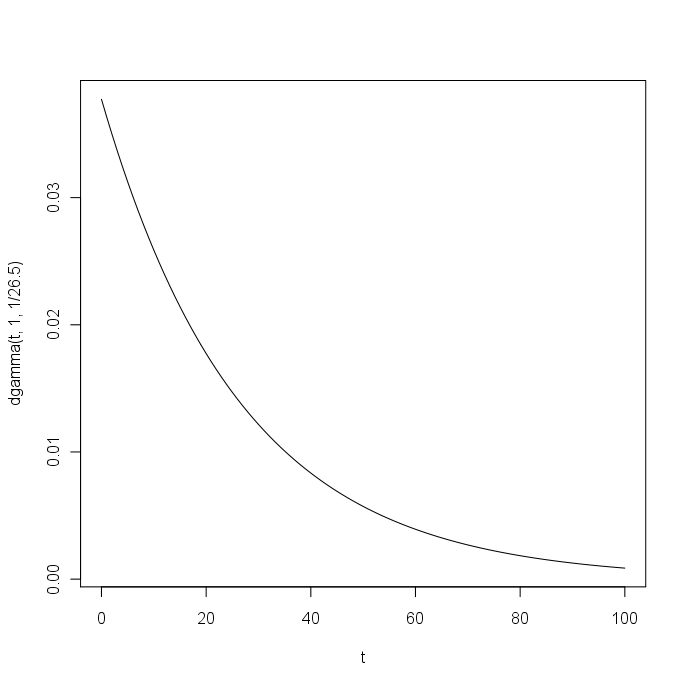
\includegraphics[width=3.3in,height=3.3in]{images/2_5-dgamma.png}\\
	Funci\'on de distribucion:\\
  	  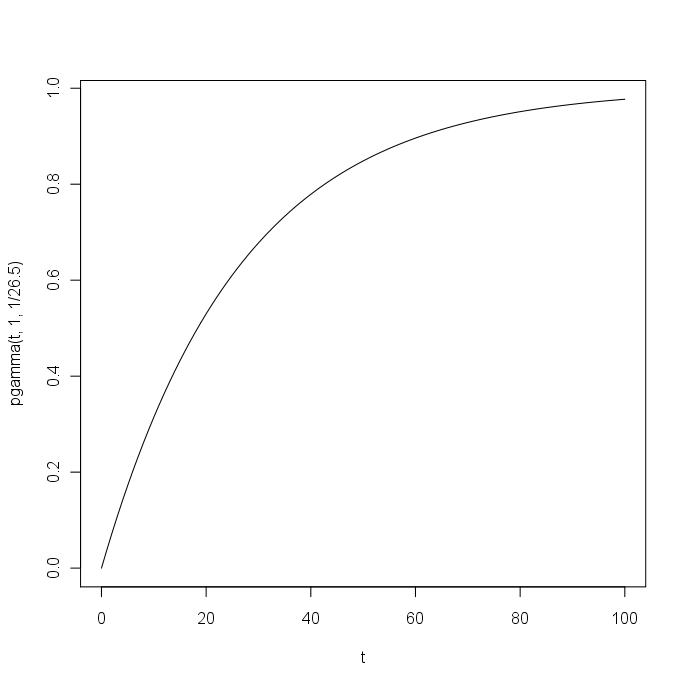
\includegraphics[width=3.3in,height=3.3in]{images/2_5-pgamma.png}
	
\end{itemize}
